\documentclass[10pt]{article}
\usepackage[margin=1in, paperwidth=8.5in, paperheight=11in]{geometry}
\usepackage{ifpdf,amsmath, amssymb, comment, color, graphicx, stmaryrd,setspace,enumitem,tikz, fancyhdr, wrapfig, textcomp, mathptmx, siunitx}


\usepackage{hyperref}
\hypersetup{
    colorlinks=true,
    urlcolor=blue,
}

\setlength{\headheight}{14.5pt}
\newcommand{\Q}{\mathbb{Q}}
\newcommand{\R}{\mathbb{R}}
\newcommand{\Z}{\mathbb{Z}}
\newcommand{\vu}{\mathbf{u}}
\newcommand{\vv}{\mathbf{v}}
\newcommand{\vw}{\mathbf{w}}
\newcommand{\vi}{\mathbf{i}}
\newcommand{\vj}{\mathbf{j}}
\newcommand{\vk}{\mathbf{k}}
\newcommand{\vn}{\mathbf{n}}
\newcommand{\vr}{\mathbf{r}}
\newcommand{\proj}{\operatorname{proj}}
\newcommand{\orth}{\operatorname{orth}}
\newcommand{\comp}{\operatorname{comp}}
\newcommand\dotp[1][.5]{\,\mathbin{\vcenter{\hbox{\scalebox{#1}{$\bullet$}}}}\,}
	
% Solution text is in red. If you want the solutions to show, remove the \iffalse from the definition of the \red command.
\newenvironment{red}{\color{red}}{\ignorespacesafterend}
\newcommand{\blue}[1]{\textcolor{blue}{#1}}
\newcommand{\green}[1]{\textcolor{green}{#1}}
\renewcommand{\section}[1]{\begin{center} \textbf{#1} \\\end{center}}
%
\hyphenpenalty=5000
\setlength{\parindent}{0in}
%\oddsidemargin=-.25in
\allowdisplaybreaks
\pagestyle{fancy}
\renewcommand{\headrulewidth}{0pt}
\lhead{MATH 203}
\rhead{Fall 2024}
%\lfoot{\copyright\ CLEAR Calculus 2010}
\cfoot{}

\begin{document}
%


%\onehalfspacing
\allowdisplaybreaks
%##################################################################
\section{PS\#3: Lines and planes - \red{Answer key} }

\begin{enumerate}[leftmargin=0pt]

\item (\href{https://activecalculus.org/multi/S-9-5-Lines-Planes.html#Ez_9_5_1}{AC Multi 9.5 Exercise 10})  The vector and parametric forms of a line allow us to easily describe line segments in space.

Let $P_1 = (1, 2, -1)$ and $P_2 = (-2, 1, 2)$, and let $\mathcal{L}$ be the line in $\R^3$ through $P_1$ and $P_2$, as in Activity 9.5.2. 
\begin{red}
	As a reminder, we decided that the line $\mathcal{L}$ has the vector equation $\vr(t) = \langle 1, 2, -1 \rangle + t\,\langle -3, -1, -1 \rangle$.
\end{red}
\begin{enumerate}
	\item What value of the parameter $t$ makes $(x(t), y(t), z(t)) = P_1$? What value of $t$ makes $(x(t), y(t), z(t)) = P_2$? 
	
	\begin{red}
		In this parameterization of the line, $t=0$ corresponds to $P_1$ and $t=1$ corresponds to $P_2$.
	\end{red}
	\item What $t$ values describe the line segment between the points $P_1$ and $P_2$?
	
	\begin{red}
		Unsurprisingly, the $t$ values between 0 and 1: $t\in[0, 1]$, or in other words $0 \leq t \leq 1$.
	\end{red}
	\item What about the line segment (along the same line) from $(7,4,1)$ to $(-8, -1, -4)$?
	
	\begin{red}
		The point $(7,4,1)$ corresponds to $t = -2$ and the point $(-8, -1, -4)$ corresponds to $t = 3$. Therefore, this segment corresponds to the $t$ values $-2 \leq t \leq 3$.
	\end{red}
	\item Now, consider a segment that lies on a different line: parameterize the segment that connects point $R=(4, -2, 7)$ to $Q = (-11, 4, 27)$ in such a way that $t=0$ corresponds to point $Q$, while $t=2$ corresponds to $R$.
	
	\begin{red}
		If we want $t=0$ to correspond to point $Q$, then we should use the vector $\overrightarrow{OQ} = \langle -11, 4, 28 \rangle$ as our initial vector $\vr_0$. Then the direction vector should be in the direction of $\overrightarrow{QP} = \langle 4-(-11), -2-4, 7-27 \rangle = \langle 15, -6, -20\rangle$. 
		
		However, if we just used that vector as-is, then the point $P$ would correspond to $t=1$. Let us therefore cut $\overrightarrow{QP}$ in half. The vector equation of this line is therefore:
		\[\vr(t) = \langle -11, 4, 27 \rangle + t\cdot\left\langle \frac{15}{2}, \frac{-6}{2}, \frac{-20}{2}\right\rangle.\]
	\end{red}
\end{enumerate}
	
\item (\href{https://activecalculus.org/multi/S-9-5-Lines-Planes.html#Ez_9_5_2}{AC Multi 9.5 Exercise 11}) This exercise explores key relationships between a pair of lines. Consider the following two lines: one with parametric equations $x(s) = 4 - 2s$, $y(s) = -2 + s$, $z(s) = 1+3s$, and the other being the line through $(-4,2,17)$ in the direction $\vv = \langle -2, 1, 5\rangle$.
\begin{enumerate}
	\item Find a direction vector for the first line, which is given in parametric form.
	
	\begin{red}
		This line points in the direction of the vector $\vw = \langle -2, 1, 3\rangle$.
	\end{red}
	\item Find parametric equations for the second line, written in terms of the parameter $t$.
	
	\begin{red}
		$x(t) = -4 - 2t$, $y(t) = 2+1t$, and $z(t) = 17+5t$.
	\end{red}
	\item Show that the two lines intersect at a single point by finding the values of $s$ and $t$ that result in the same point. Then find the point of intersection.
	
	\begin{red}
		We want to solve the system of equations:
		\begin{align*}
			4 - 2s &= -4 - 2t \\
			-2 + s &= 2 + 1t \\
			1 + 3s &= 17 + 5t
		\end{align*}
		A bit of boring algebra that I won't reproduce here leads us to the solution $s = -2$, $t = -2$. Both $s = 2$ and $t = -2$ correspond to the point $(0, 0, 7)$ (check!).
	\end{red}
	\item Find the acute angle formed where the two lines intersect, noting that this angle will be given by the acute angle between their respective direction vectors.
	
	\begin{red}
		\begin{align*}
			\cos\theta &= \dfrac{\vv \dotp \vw}{|\vv|\cdot|\vw|}
			= \dfrac{\langle -2, 1, 5 \rangle \dotp \langle -2, 1, 3 \rangle}{\sqrt{(-2)^2 + 1^2 + 5^2} \cdot \sqrt{(-2)^2 + 1^2 + 3^2}} = \dfrac{4 + 1 + 15}{\sqrt{30} \cdot \sqrt{14}} = \dfrac{20}{\sqrt{420}} \\
			\theta &= \arccos\left(\dfrac{20}{\sqrt{420}}\right)\approx 0.21999 \approx 12.604^\circ 
		\end{align*}
	\end{red}
	\item Find an equation for the plane that contains both of the lines described in this problem.
	
	\begin{red}
		A normal vector is given by the cross product:
		\[\vn = \vv\times\vw =  \langle -2, 1, 5 \rangle \times \langle -2, 1, 3 \rangle = \langle 2, 4, 0 \rangle\]
		A point on the plane is the one we found in part (c), which is $(0, 0, 7)$. Therefore, an equation for the plane is 
		\[ 2(x-0) + 4(y-0) + 0(z-7) = 0. \]
		(Your equation may of course be different from mine, particularly if you computed $\vw\times\vv$ instead of $\vv\times\vw$.)
	\end{red}
\end{enumerate}

\item (\href{https://activecalculus.org/multi/S-9-5-Lines-Planes.html#Ez_9_5_3}{AC Multi 9.5 Exercise 12}) This exercise explores key relationships between a pair of planes. Consider the following two planes: one with scalar equation $4x-5y+z = -2$, and the other which passes through the points $(1,1,1)$, $(0, 1, -1)$, and $(4, 2, -1)$.
\begin{enumerate}
	\item Find a vector normal to the first plane.
	
	\begin{red}
		We can just read it off from the scalar equation: the vector $\langle 4, -5, 1\rangle$ is normal to the plane.
	\end{red}
	\item Find a scalar equation for the second plane.
	
	\begin{red}
		This will require some more computation. First, we need to turn our three points into two vectors that go between them. (Your work may be a little different from mine here, because you might subtract the vectors in a different order, and that's okay.)\\
		Let's say that $\vu$ is the vector from $(1,1,1)$ to $(0,1,-1)$, so $\vu = \langle-1, 0, -2\rangle.$\\
		Let's say that $\vv$ is the vector from $(1,1,1)$ to $(4, 2, -1)$, so $\vv = \langle 3, 1, -2 \rangle.$\\
		Then we can get a normal vector $\vn$ by finding the cross product (this sounds like a good job for Wolfram$|$Alpha): $\vn = \langle 2, -8, -1 \rangle$. \\
		Now let's identify one of the points as $P_0$ so that we can write down the vector equation of the plane, and then we can translate the vector equation into a scalar equation. I'll say $P_0 = (1, 1, 1)$, so that $\overrightarrow{PP_0} = \langle x-1, y-1, z-1\rangle$.\\
		Then the vector equation is:
		\begin{align*}
			\vn\dotp\overrightarrow{PP_0} &= 0 \\
			\langle 2, -8, -1 \rangle \dotp \langle x-1, y-1, z-1\rangle &= 0 \\
			2(x-1) -8(y-1) -1(z-1) &= 0 
			\intertext{This is certainly good enough, but we can simplify a little more if we want:}
			2x - 2 -8y +8 -z + 1 &= 0 \\
			2x -8y -z +7 &= 0 \\
			2x - 8y - z &= -7
		\end{align*}
	\end{red}
	\item Find the angle between the planes, where the angle between them is defined by the angle between their respective normal vectors.
	
	\begin{red}
	Let's call the two normal vectors $\vn_1$ and $\vn_2$. Since $\vn_1 \dotp \vn_2 = |\vn_1|\cdot|\vn_2| \cdot \cos\theta$, where $\theta$ is the angle between the vectors, we can use the dot product to compute the angle between the vectors:
		\begin{align*}
			\cos\theta &= \frac{\vn_1 \dotp \vn_2}{|\vn_1|\cdot|\vn_2|} 
			= \frac{\langle 4, -5, 1\rangle \dotp \langle 2, -8, -1 \rangle }{|\langle 4, -5, 1\rangle| \cdot |\langle 2, -8, -1 \rangle|}\\
			&= \frac{4\cdot 2 + (-5)\cdot(-8) + 1 \cdot (-1)}{\sqrt{4^2 + (-5)^2 + 1^2} \cdot \sqrt{2^2 + (-8)^2 + (-1)^2}}\\
			&= \frac{47}{\sqrt{42}\cdot\sqrt{69} } \\
			\theta &= \arccos\left(\frac{47}{\sqrt{42}\cdot\sqrt{69}}\right)\\
			&\approx 0.509 \quad (\approx 29.18^\circ)
		\end{align*}
	\end{red}
	\item Find a point that lies on both planes.
	
	\begin{red}
		Let's solve both scalar equations for $z$, and then equate the two $z$'s. 
		\begin{align*}
			\textrm{Plane 1: } 4x - 5y + z &= -2 \\
			z &= -2 -4x + 5y \\
			\textrm{Plane 2: } 2x - 8y - z &= -7 \\
			z &= 2x - 8y + 7 \\
			-2 - 4x + 5y &= 2x - 8y + 7 \\
			6x -13y &= -9
			\intertext{Now we get to pick some value we want for one of these variables. How about $x=0$?}
			-13y &= -9 \\
			y &= \dfrac{9}{13}
			\intertext{Cool, so now we have the $x$- and $y$-coordinates of a point that's on both planes. Substituting back into one of our $z$ equations:}
			z &= -2 -4x +5y \\
			&= -2 -4(0) + 5\left(\dfrac{9}{13}\right) = \dfrac{19}{13}
		\end{align*}
		Therefore, $\left(0, \dfrac{9}{13}, \dfrac{19}{13}\right)$ is a point that lies on both planes.

		(Other points that work include $\left(-\dfrac32, 0, 4\right)$, $\left(\dfrac{19}{22}, \dfrac{12}{11}, 0\right)$, and $(5,3,-7)$.)

	\end{red}
	\item Since these two planes do not have parallel normal vectors, the planes must intersect, and thus must intersect in a line. Observe that the line of intersection lies in both planes, and thus the direction vector of the line must be perpendicular to each of the respective normal vectors of the two planes. Find a direction vector for the line of intersection for the two planes.
	
	\begin{red}
		If we want a direction vector $\vv$ who's perpendicular to both of our two normal vectors $\vn_1$ and $\vn_2$, why don't we use the cross product? \\
		$\vv = \vn_1 \times \vn_2 = \langle 4, -5, 1\rangle \times \langle 2, -8, -1 \rangle = \langle 13, 6, -22 \rangle$ (Thanks, W$|$A!)
	\end{red}
	\item Determine parametric equations for the line of intersection of the two planes.
	
	\begin{red}
		Alls we need is a direction vector and a point. But hey, we've got both of those! \\
		$\mathbf{L}(t) = \mathbf{r}_0 + t \vv 
		= \langle 0, \tfrac{9}{13}, \tfrac{19}{13} \rangle 
		+ t \langle 13, 6, -22 \rangle
		= \langle 0 + 13t, \tfrac{9}{13} + 6t, \tfrac{19}{13} - 22t \rangle$ \\
		In parametric form:
		\begin{align*}
			x(t) &= 13t\\
			y(t) &= \tfrac{9}{13} + 6t\\
			z(t) &= \tfrac{19}{13} - 22t
		\end{align*}
	\end{red}
\end{enumerate}

\item  (AC Multi 9.5 Exercise 13) In this problem, we explore how we can use what we know about vectors and projections to find the distance from a point to a plane. Let $p$ be the plane with equation $z=-4x+3y+4$, and let $Q = (4, -1, 8)$
\begin{enumerate}
    \item Show that $Q$ does not lie in the plane $p$.
    
    \begin{red}
    If $Q$ was in the plane $p$, then the coordinates of $Q$ would satisfy the scalar equation of $p$. Let's substitute the coordinates of $Q$ into the equation for $p$ and see if we win.
    \[8 = -4\cdot 4 + 3\cdot (-1) + 4 = -16 - 3 + 4 = -15,\]
    which is certainly not true, so $Q$ does not lie in $P$.
    \end{red}
    \item Find a normal vector $\vn$ to the plane $p$.
    
    \begin{red}
    Let's rearrange the equation for $p$ to put it in the usual form $ax + by + cz = d$. Then we can read the normal vector right off the coefficients of $x$, $y$, and $z$. We get
    \[-4x + 3y - z = -4,\] so the normal vector is $\vn = \langle -4, 3, -1\rangle$. (Of course, $\langle 4, -3, 1\rangle$ would also work.)
    \end{red}
    \item Find the coordinates of a point $P$ in $p$.
    
    \begin{red}
    We sort of get to just pick any point we want, so let's pick an easy one where the $x$ and $y$ coordinates are both zero. Then $0 + 0 - z = -4$, so $z=4$. Therefore, $P = (0, 0, 4)$ is a point on $p$. (Your point may of course differ.)
    \end{red}
    \item Find the components of $\overrightarrow{PQ}$. Draw a picture to illustrate the objects found so far.
    
    \begin{red}
    $\overrightarrow{PQ} = \langle 4-0, -1-0, 8-4\rangle = \langle 4, -1, 4 \rangle$.
    
    In the picture below, I've also drawn in the shadow that $\overrightarrow{PQ}$ casts on the plane, and in red, I've drawn $\proj_\vn \overrightarrow{PQ}$.
    \end{red}
    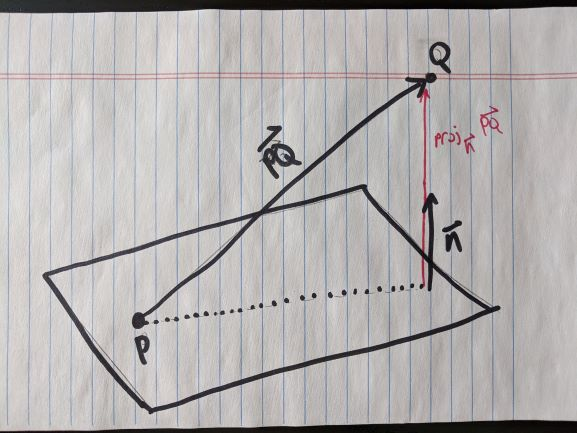
\includegraphics{../images/9-5-13.jpg}
    \item Explain why $|\comp_\vn \overrightarrow{PQ}|$ gives the distance from the point $Q$ to the plane $p$. Find this distance.
    
    \begin{red}
    $\comp_\vn \overrightarrow{PQ}$ is (basically) the length of $\proj_\vn \overrightarrow{PQ}$, so it's the length of the red vector in the picture. That's the distance from $Q$ to the point on the plane $p$ that's closest to $Q$, which is a reasonable way to define the distance between a point and a plane.
    
    (I say ``basically'' because $\comp_\vn \overrightarrow{PQ}$ is allowed to be negative. In the picture above, if $\vn$ pointed the opposite direction (that is, down from the plane rather than up off the plane), then $\comp_\vn \overrightarrow{PQ}$ would be negative. That's why we're taking the absolute value -- because all we care about is distance, we're going to ignore the sign.)
    \begin{align*}
        \comp_\vn \overrightarrow{PQ} &= \frac{\overrightarrow{PQ}\dotp \vn}{|\vn|} 
        = \frac{\langle 4, -1, 4 \rangle \dotp \langle -4, 3, -1\rangle}{|\langle -4, 3, -1\rangle|} \\
        &= \frac{-16-3-4}{\sqrt{4^2 + 3^2 + 1^2}} = \frac{-23}{\sqrt{26}}
    \end{align*}
    Oh, look, that did indeed end up being negative -- I should have drawn $\vn$ pointing the other way off the plane in the picture above -- so we should indeed take the absolute value.
    \[|\comp_\vn \overrightarrow{PQ}| = \frac{23}{\sqrt{26}} \approx 4.5107.\]
    \end{red}
\end{enumerate}

\end{enumerate}
	
\end{document}